%! Author = mboehme
%! Date = 20.03.2023

\section{Anhang}\label{sec:anhang}
\centering
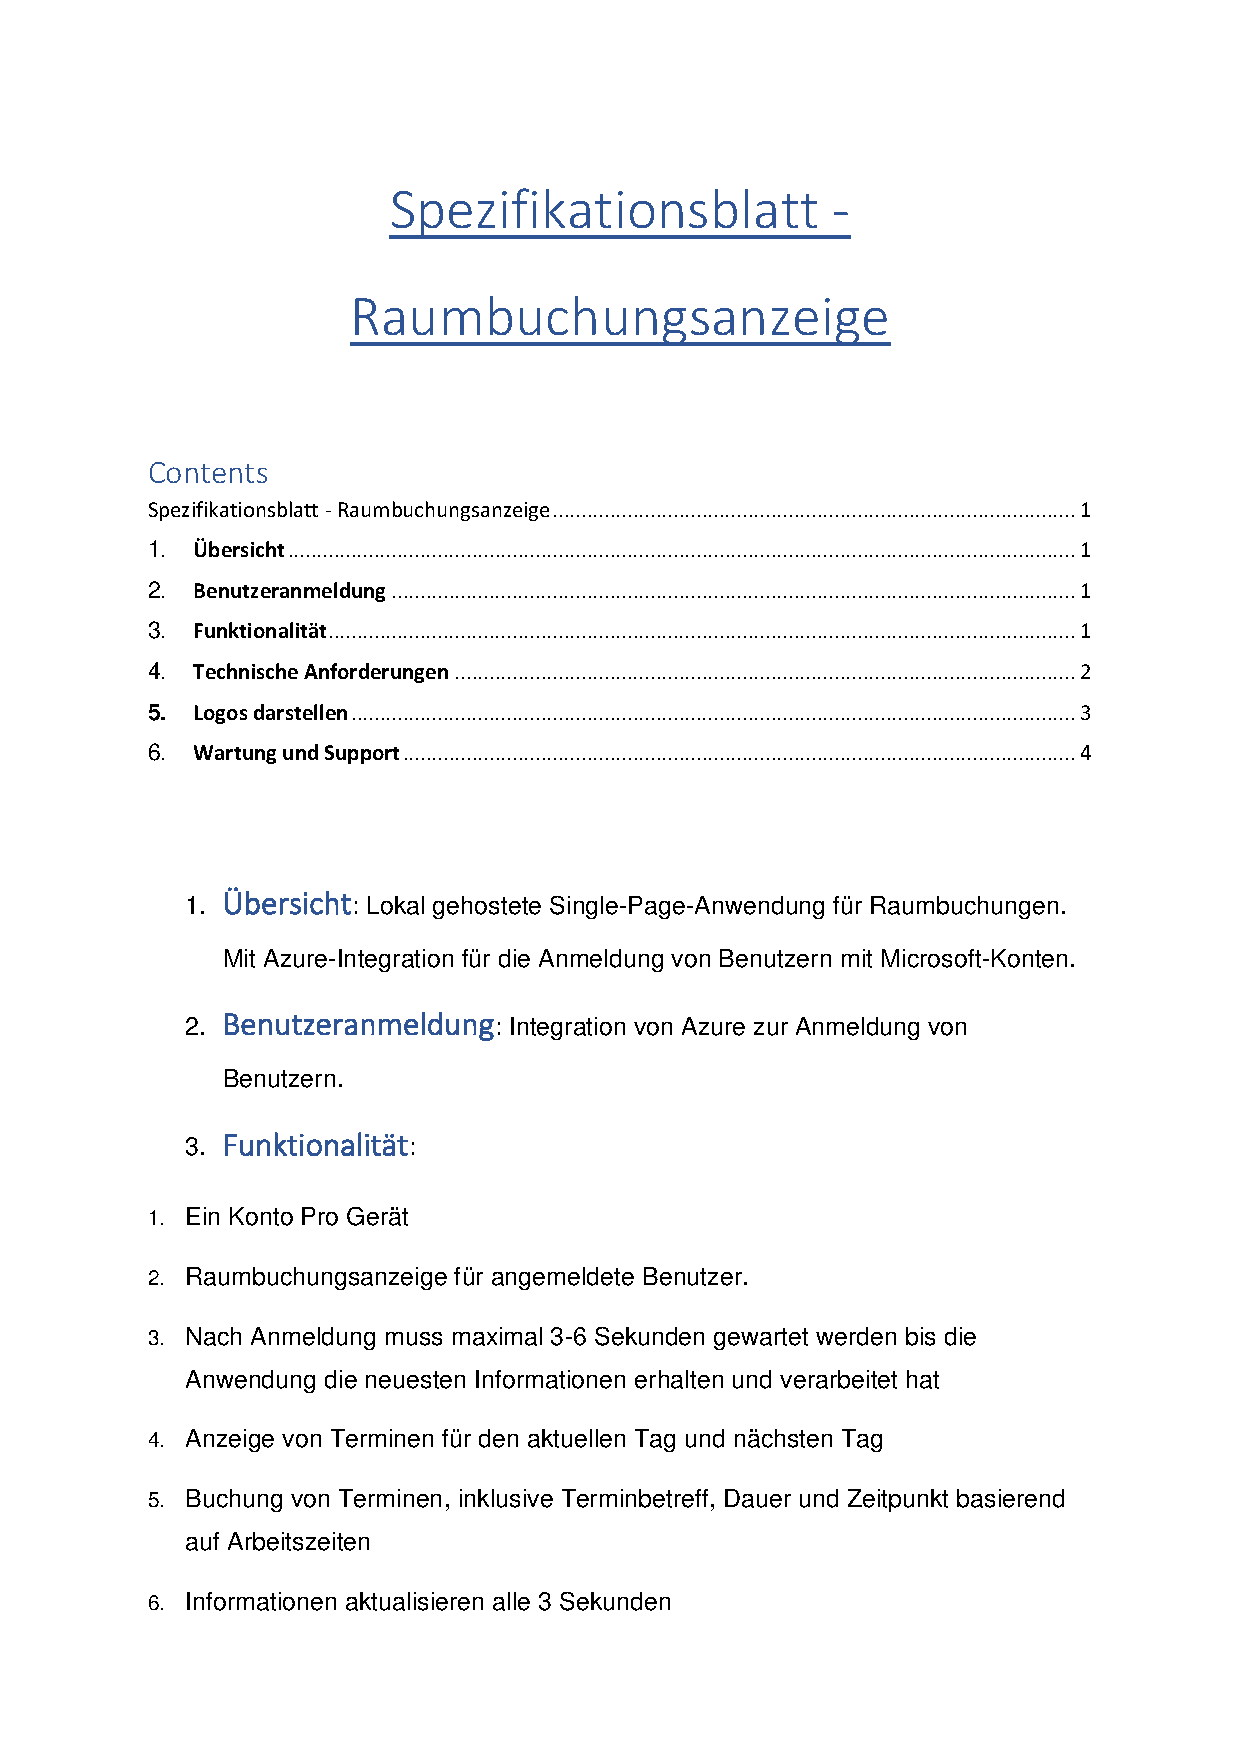
\includepdf[pages=1,pagecommand={},scale=0.8,pagecommand={\subsection{Spezifikationsblatt}\label{subsec:spezifikationsblatt}}, width=\textwidth]{PDFs/Spezifikationsblatt - Raumbuchungsanzeige - Office365 room booking - censored details.pdf}
\includepdf[pages={2-}, scale=0.8]{PDFs/Spezifikationsblatt - Raumbuchungsanzeige - Office365 room booking - censored details.pdf}
\caption{Spezifikationsblatt für die Anwendung}
\label{fig:spezifikationsblatt}
\newline
\newline
\subsection{Ablauf der Entwicklung}\label{subsec:ablauf-der-entwicklung}
Nachdem der erste Prototyp fertig war und Rücksprache gehalten wurde, wurde angefangen die Anwendung zu entwickeln.
Design und Funktionalität wurden dabei partiell parallel entwickelt, wobei die Funktionalität immer Priorität hatte.
In über 95 Commits wurden die Änderungen an der Anwendung festgehalten.
\newline
Es wurde ein Testgerät benötigt, um die Anwendung zu testen.
Ein Phillips 10BDL4551T/00 Bildschirm wurde dafür an die Wand gehängt und mit dem Internet verbunden.
Die Internetverbindung ist notwendig, um die Rest-Anfragen zwischen der Anwendung und der Microsoft Graph API zu ermöglichen.
Es wurde so eingerichtet, wie es auch beim Kunden laufen soll.
\newline
Die Anwendung wurde täglich aktiv genutzt, um so Fehler zu finden und Feedback zu geben.
Das Feedback wurde dann evaluiert.
Solche explorativen Tests sind sehr wichtig, um Intuitivität und Benutzerfreundlichkeit zu gewährleisten.
Es war einerseits hilfreich, um vorgesehene Abläufe zu testen, andererseits aber auch um Fehler zu finden, die nicht vorgesehen waren, indem Monkey Testing~\cite{Monkey-Testing-Book1} betrieben wurde.
\newline
